\section{Automatyzacja a branża IT}
\subsection{Charakteryzacja branży IT}
W 2001 roku doszło do jednej z bardziej znaczących publikacji dla szeroko pojętego biznesu IT. Został wtedy opublikowany \textit{Manifesto for Agile Software Development} autorstwa między innymi Kenta Becka, Roberta C. Martina oraz Martina Fowlera. Manifest ten opisywał rewolucyjne jak na tamte czasy praktyki \cite{AgileManifesto}:
\begin{itemize}
    \item Satysfakcja klienta dzięki wczesnemu i ciągłemu dostarczaniu oprogramowania,
    \item Zmiany wymagań mile widziane nawet na późnym etapie programowania,
    \item Częste dostarczanie działającej wersji oprogramowania (bardziej tygodnie niż miesiące),
    \item Bliska kooperacja między programistami a ludźmi zajmującymi się biznesem,
    \item Projekty powstają wokół zmotywowanych osób, którym należy ufać,
    \item Komunikacja w cztery oczy jest najlepszą formą komunikacji,
    \item Działający produkt jest najlepszym wskaźnikiem postępu prac,
    \item Zrównoważony rozwój, pozwalający na utrzymanie stałego tempa tworzenia aplikacji,
    \item Ciągła dbałość o doskonałość techniczną i dobry design,
    \item Prostota - sztuka projektowania systemu bez dużej komplikacji systemu,
    \item Najlepsze architektury, wymagania i designy powstają dzięki samoorganizującym się zespołom,
    \item Zespół regularnie zastanawia się, jak zwiększyć skuteczność i odpowiednio się dostosowuje.
\end{itemize}
Propozycje przedstawione przez autorów manifestu były dużą zmianą w stosunku do podejścia używanego powszechnie w tamtych czasach.
\par
W latach 80 oraz 90 XX wieku popularnie stosowaną techniką była metodologia Waterfall, zobrazowana na rysunku \ref{fig:waterfall}.
\begin{figure}[htbp]
    \centering
    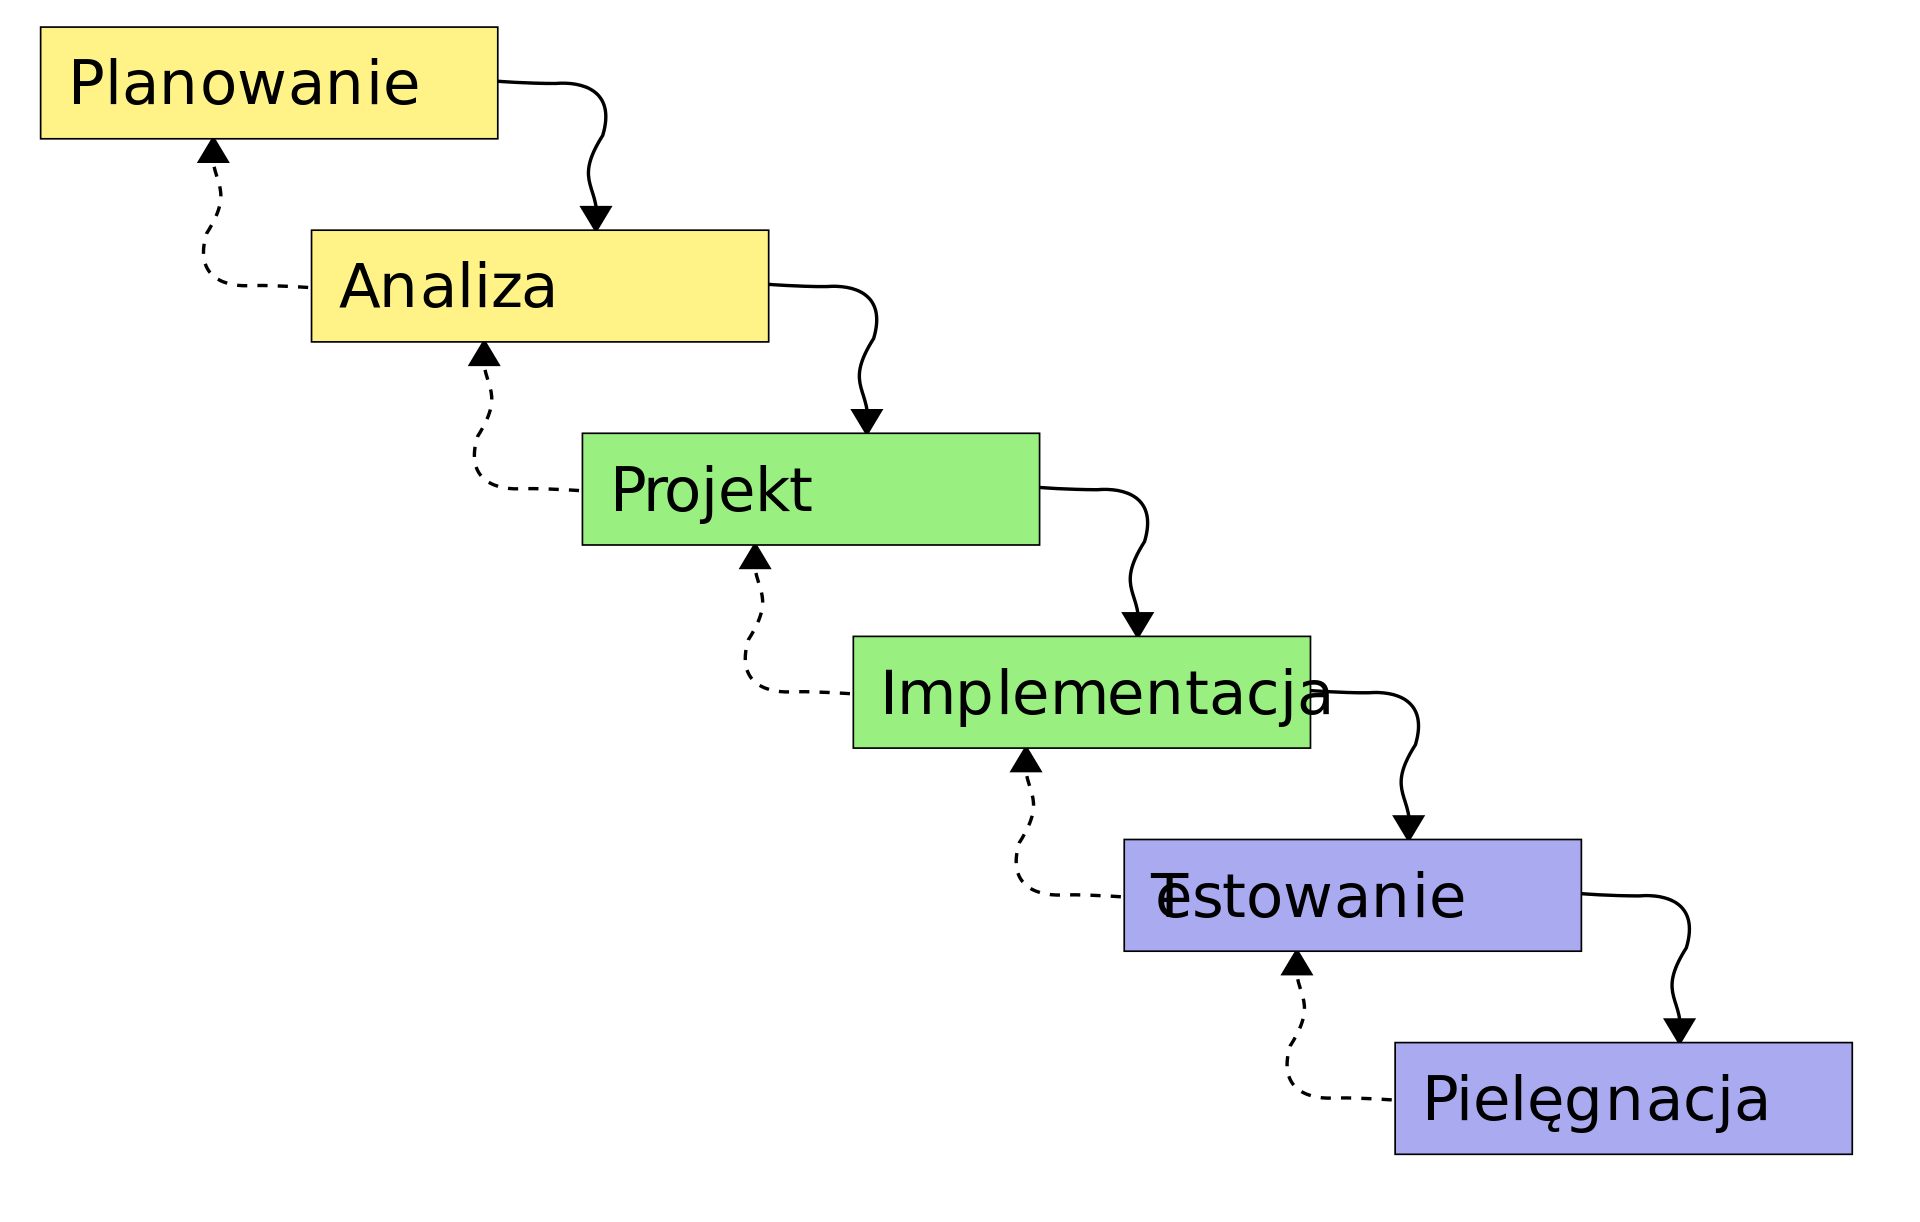
\includegraphics[width=10cm]{waterfall.png}
    \caption{Metodologia Waterfall}
    \label{fig:waterfall}
\end{figure}
Poszczególne etapy projektowe były wykonywane tylko raz podczas procesu tworzenia oprogramowania. Z tego faktu wszelakie zmiany na późniejszym etapie projektowym były trudne w realizacji. Konkurencja na rynku oprogramowania komputerowego była na tyle niewielka, że producenci oprogramowania nie musieli przejmować się zanadto uwagami od użytkowników - to sprawiało, że Waterfall spełniał swoje zadania. 
\par
Pierwsze dziesięciolecie XXI wieku spopularyzowało jedno z największych osiągnięć ludzkości - Internet. Nowa rzeczywistość, w której ludzkość coraz więcej czasu spędza przed urządzeniami elektronicznymi postawiła przez twórcami oprogramowania nowe wymagania. Dodatkowo coraz większe grono przedsiębiorców zaczyna dostrzegać w produkcji oprogramowania zyski. Użytkownicy zaczynają coraz bardziej spoglądać na przyjemny dla oka wygląd oprogramowania oraz jego prostotę. Metodyka zaproponowana przez autorów manifestu Agile zdaje się świetnie wpisywać w wizję tworzenia oprogramowania na miarę nowego tysiąclecia.
\par
Jedną z bardziej znanych implementacji Agile jest metodologia o nazwie Scrum.
\begin{figure}[htbp]
    \centering
    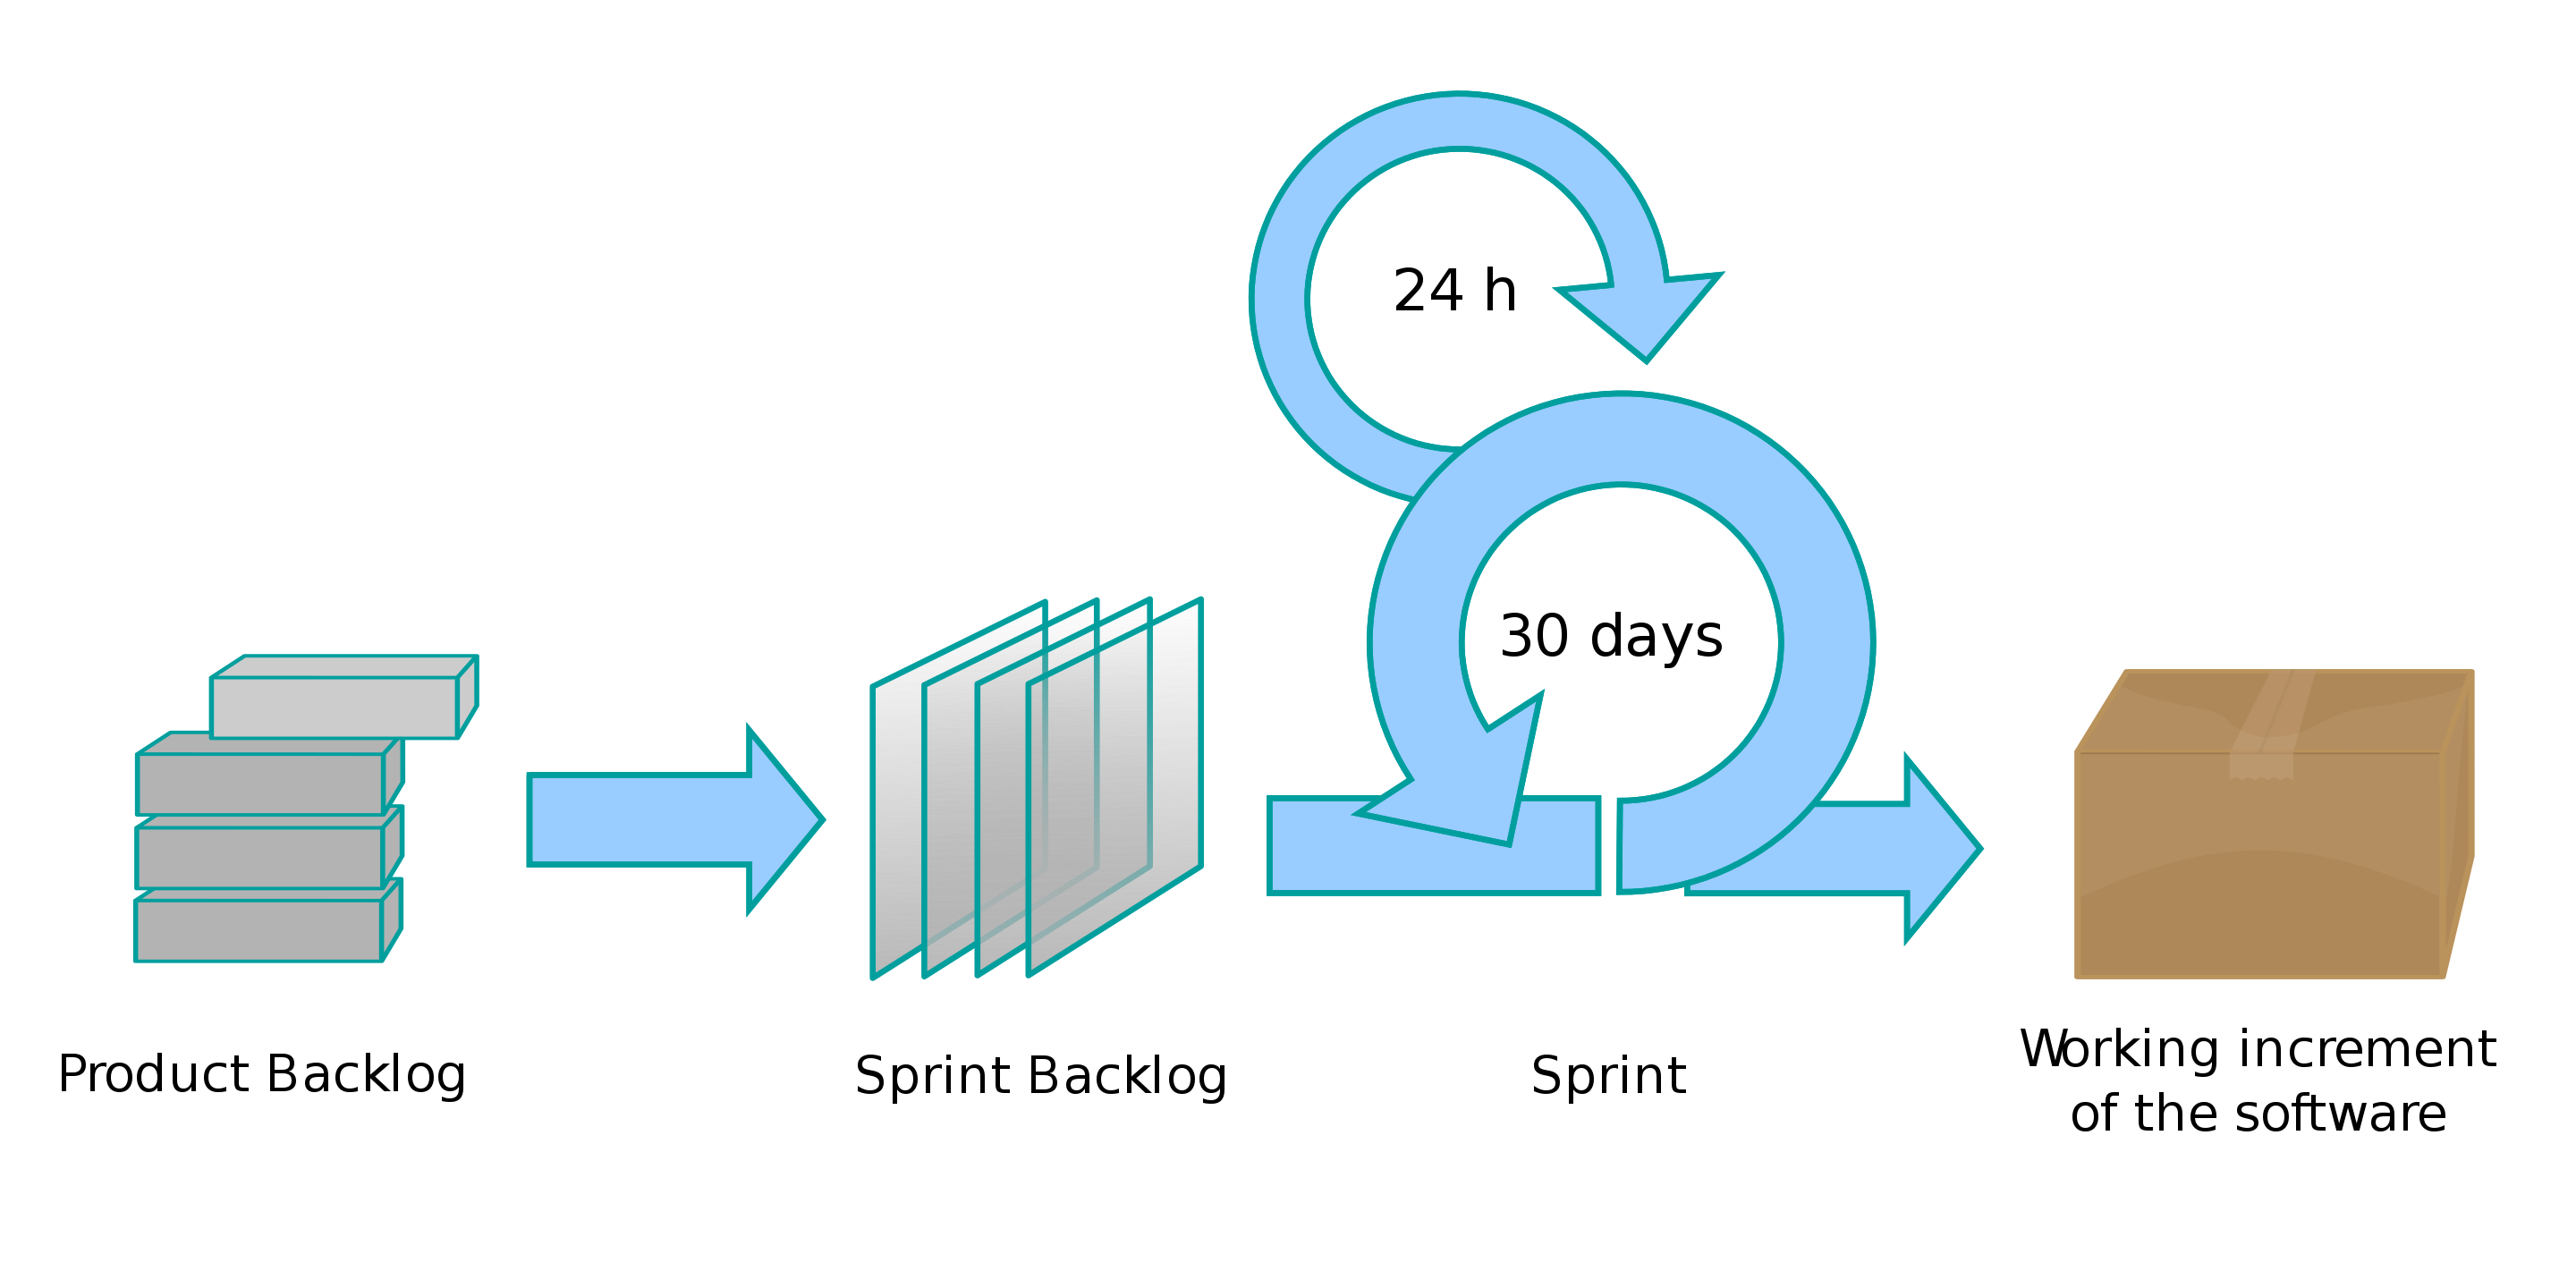
\includegraphics[width=10cm]{scrum.png}
    \caption{Framework Scrum}
    \label{fig:scrum}
\end{figure}
Zakłada się w niej, że oprogramowanie powstaje w procesie kolejnych inkrementacji. Każda iteracja jest nazywana sprintem. Sprint ma z góry zdefiniowane ramy czasowe, w których będzie on trwał. Na podstawie różnych czynników biznesowych opiekun projektu decyduje, które zadania powinny trafić do danego sprintu, a które są mniej priorytetowe i mogą pozostać w tzw. backlogu. Efektem końcowym danego sprintu jest działający produkt, który jest wzbogacony o rzeczy dodane podczas trwania sprintu. Scrum sam w sobie nie narzuca, ile powinien trwać dany sprint, czy też jaki system powinien być stosowany do śledzenia zadań. Wszystko zależy od preferencji danego zespołu programistycznego. Integralną częścią każdego sprintu jest retrospektywa. Na takim spotkaniu zespół dyskutuje jakie zmiany należy dokonać w procesie, by uefektywnić pracę. Dzięki elastycznemu podejściu i możliwości ulepszania procesu Scrum wydaje się być dobrym rozwiązaniem dla zespołów, które wypuszczają oprogramowanie regularnie oraz zmieniają je na podstawie opinii użytkowników.
\subsection{Agile a automatyzacja}
Spełnienie wymagań wymienionych w manifeście Agile wydaje się być trudne w kontekście częstego wypuszczania działającej wersji. Oczekuje się tego, aby zespół deweloperski regularnie publikował działającą wersję podglądową oprogramowania dla osób nietechnicznych. Problem ten można rozwiązać na co najmniej dwa sposoby:
\begin{itemize}
    \item Manualny - Członek zespołu deweloperskiego regularnie według wymagań zajmuje się budowaniem wersji podglądowej oraz udostępnia ją osobom zainteresowanym,
    \item Automatyczny - Zespół deweloperski ustawia automatyczne procesy, które na serwerze budującym tworzą wersję podglądową aplikacji oraz publikują ją dla osób zainteresowanych.
\end{itemize}
Proces automatyczny jest preferowanym sposobem publikacji oprogramowania. Ma on kilka zalet nad sposobem manualnym. Nie tracimy czasu specjalisty, który musiałby poświęcić go na zbudowanie i publikację aplikacji. Drugą zaletą jest fakt, że serwer za każdym razem robi te same kroki podczas procesu budowania. Tym sposobem wykluczamy możliwość popełnienia błędu przez człowieka.
\par
Dobre praktyki związane z częstym budowaniem podglądowej wersji oprogramowania są określane jako DevOps. Len Bass, Ingo Weber oraz Liming Zhu w swojej książce \cite{DevOpsBook} określają DevOps jako zbiór praktyk których celem jest zmniejszenie czasu publikacji zmian na serwerze produkcyjnym przy jednoczesnej trosce o wysoką jakość. W praktyce często członkiem zespołu deweloperskiego jest tzw. DevOps. Jego zadaniem jest automatyzacja wszelakich procesów oraz często także utrzymanie środowiska produkcyjnego. Osoba na tym stanowisku powinna się cechować dobrą znajomością systemu operacyjnego, który jest używany na serwerach produkcyjnych oraz deweloperskich. Ponadto powinna być zorientowana w różnych rozwiązaniach chmurowych które współcześnie są coraz częściej używane.
\subsection{Git - kamień milowy dla deweloperów}
Ciężko byłoby sobie wyobrazić obraz dzisiejszego przemysłu IT, gdyby nie system kontroli wersji Git. Jego autorem jest Linus Torvalds. Co ciekawe stworzył on Git'a jako dodatkowy projekt, który miał pomóc w pisaniu jądra Linuxa. Dzięki Git'owi każdy członek zespołu deweloperskiego ma dostęp do wspólnego repozytorium, gdzie każdy może publikować swoje zmiany. Jedną z ważniejszych funkcji Git'a jest możliwość tworzenia własnych rozgałęzień kodu, gdzie dany programista wysyła swoje zmiany. Dalej w procesie merge'owania jest możliwe połączenie zmian danego dewelopera z kodem innych programistów. Dzięki tej cesze Git nadaje się świetnie do wszelakich projektów programistycznych, w których pracuje kilku programistów równolegle. Z biegiem lat Git stał się standardem.
\par
Powszechnie znaną dobrą techniką związaną z strukturą tego, co mamy na Gicie jest tzw. \textit{Git Workflow}. Wzorzec ten sugeruje, by używać 2 głównych gałęzi. Jedną, która będzie odzwierciedlała finalną, zdatną do użytku wersję oraz drugą, gdzie znajduje się wersja deweloperska. Pośrednie gałęzie służą do implementacji poszczególnych nowych funkcjonalności oraz do synchronizacji wersji deweloperskiej z gałęzią produkcyjną. Dzięki takiemu podejściu proces deployment'u na środowisko produkcyjne oraz testowe staje się o wiele prostszy, ponieważ mamy dwie gałęzie, które odzwierciedlają te środowiska. Na rysunku \ref{fig:git} możemy podejrzeć szczegółowy schemat, jak powinno wyglądać repozytorium Git'owe korzystające z wzorca \textit{Git Workflow}
\begin{figure}[htbp]
    \centering
    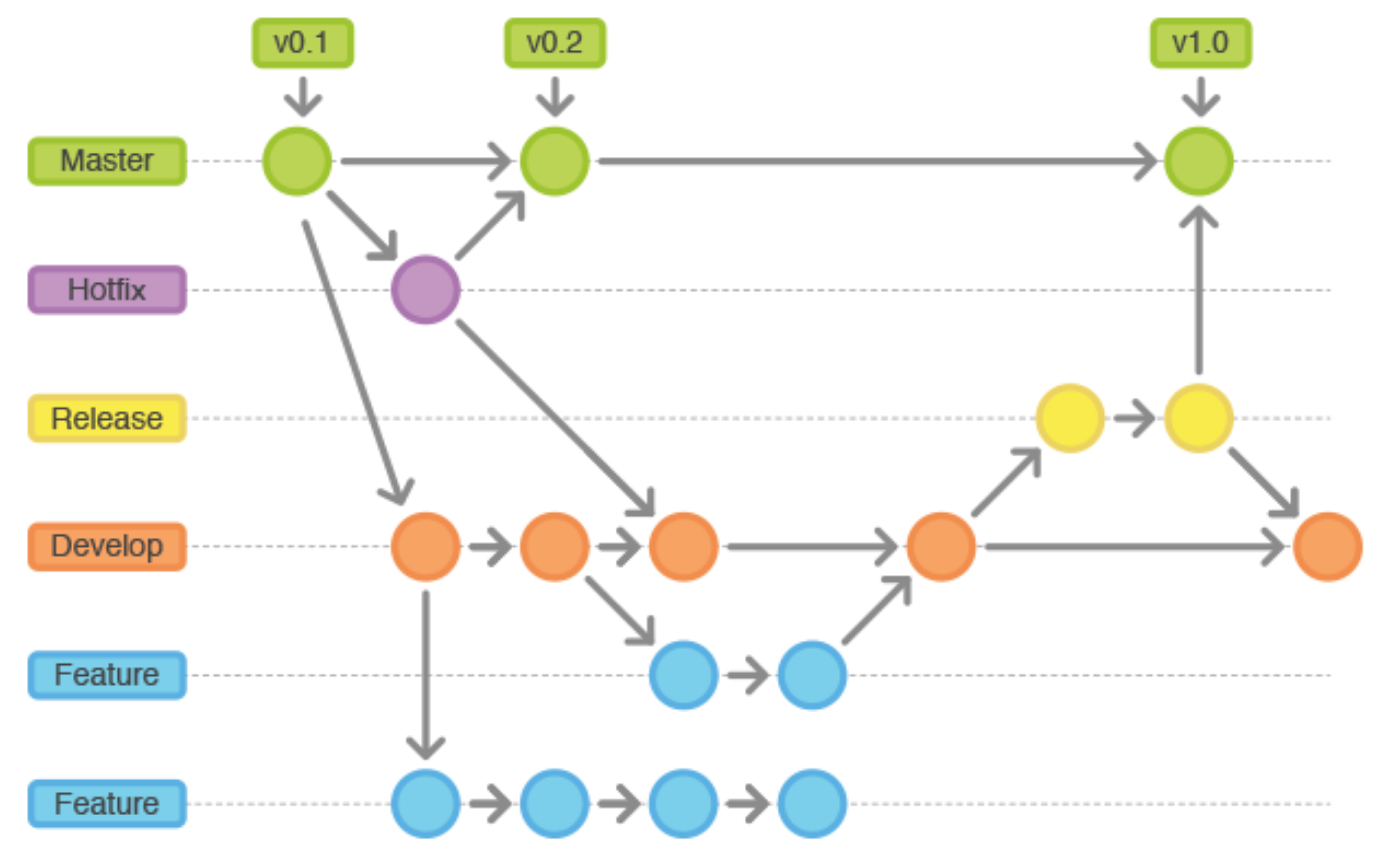
\includegraphics[width=10cm]{git.png}
    \caption{Git Workflow}
    \label{fig:git}
\end{figure}
\par
W pierwszym dziesięcioleciu XXI wieku popularne stały się rozwiązania SaaS (z ang. \textit{oprogramowanie jako usługa}) takie jak GitHub, GitLab czy też BitBucket. Dzięki takiemu rozwiązaniu nie musimy się przejmować utrzymaniem własnego serwera Git. Dodatkowo platformy SaaS zapewniają nam wszelakie aktualizacje, które usprawniają system. Platformy takie jak GitHub zapewniają narzędzia, które ułatwiają proces tworzenia oprogramowania. Narzędzia te są dopasowane, aby działać dobrze z naszym repozytorium. Przykładem takiego rozwiązania jest \textit{GitHub Pages}. Technologia ta pozwala publikować stronę www na podstawie plików, które są częścią repozytorium. Użytkownik definiuje, na której gałęzi oraz w którym folderze znajdują się pliki ze stroną internetową. Od tego momentu GitHub automatycznie stwarza nam stronę internetową dostępną pod subdomeną \textit{nazwauzytkownika.github.io}.
\subsection{Ciągła integracja}
Programiści podczas tworzenia nowych funkcjonalności powinni się upewnić, że ich zmiany nie zepsują tego, co już istnieje. Jednym z takich sposobów jest odpalenie testów. Najbardziej znanymi typami testów są:
\begin{itemize}
    \item testy jednostkowe - testy te skupiają się na testowaniu funkcji oraz klas w danym projekcie. Są najprostszą formą testowania podczas której zastępuje się wszelkie trzecie zależności tzw. \textit{mock'ami},
    \item testy integracyjne - są to testy, w których odpalany jest testowany projekt oraz wybrany projekt trzeci, z którym chcemy sprawdzić poprawność działania,
    \item testy e2e - testy te wymagają działającej w pełni aplikacji wraz z wszystkimi zależnymi projektami. Zazwyczaj sprawdzają najbardziej znaczące funkcjonalności naszej aplikacji.
\end{itemize}
Pisanie testów jest integralną częścią pracy programisty. Ich jakość oraz ilość jest znaczącym wskaźnikiem mówiącym o stanie danego projektu. Pozwalają one na tworzenie oprogramowania, które powinno mieć mniej błędów. Ciągła integracja przenosi odpowiedzialność za odpalanie testów z programisty na serwer ciągłej integracji.
\par
Testy to nie jedyna rzecz, która może być sprawdzana za pomocą ciągłej integracji. W procesie tym jest ważne, by zweryfikować jakość nowego kodu stworzonego przez developera. Przykładowymi rzeczami, które możemy zrobić podczas procesu ciągłej integracji jest:
\begin{itemize}
    \item sprawdzenie procentowego pokrycia testami projektu. Możemy na tej podstawie nie pozwolić na zmergowanie zmian, jeżeli przekroczymy z góry ustaloną procentową ilość kodu, która nie jest pokryta testami,
    \item sprawdzenie czy kod jest poprawnie sformatowany według ustalonych reguł. Proces ten nazywa się powszechnie \textit{lintowaniem}. Dzięki temu unikniemy problemu, w którym kod będzie różnie sformatowany w zależności dewelopera piszącego kod,
    \item testowanie aplikacji na niestandardowych systemach operacyjnych. Dzięki temu możemy się upewnić, że nasza aplikacja zadziała na mniej standardowych konfiguracjach. Jest to szczególnie istotne, jeżeli deweloperzy oraz testerzy nie skupiają się na testowaniu na danym systemie operacyjnym,
    \item sprawdzanie czy zależności trzecie, które są używane w projekcie nie mają żadnych podatności związanych z bezpieczeństwem aplikacji. Z racji tego możemy na wczesnym etapie wychwycić takie problemy i odpowiednio szybko zaaktualizować te biblioteki,
    \item zbudowanie obrazów dockerowych. Taki krok pozwala osobom znającym dockera bezproblemowe przetestowanie każdej gałęzi w naszym projekcie.
\end{itemize}
Dobór rzeczy, które chcemy zautomatyzować zależy od indywidualnych potrzeb danego projektu. Za duża komplikacja procesu ciągłej integracji może przynieść więcej szkody niż korzyści. Należy pamiętać, że programista musi czekać na to, aż proces ciągłej integracji się wykona.
Więcej o testach opisane jest w rozdziale 5.
\subsection{Ciągłe dostarczanie}
Podczas gdy ciągła integracja skupia się na upewnieniu, czy dane zmiany przechodzą testy, tak zadaniem procesów ciągłego dostarczania jest zbudowanie aplikacji oraz umożliwienie jej późniejszej manualnej publikacji na środowisku produkcyjnym. Każdy projekt ma swoją własną specyfikę i proces ciągłego dostarczania jest inaczej ustawiany. Punktem wspólnym jest to, że człowiek decyduje, kiedy powinno nastąpić wydanie nowej wersji oprogramowania.
\par
Zanalizujmy typowy przykład, jak może wyglądać proces ciągłej integracji. Mamy aplikację webową, która komunikuje się z bazą danych oraz wystawia API. Istnieją dwa środowiska gdzie działa ten serwis:
\begin{itemize}
    \item środowisko produkcyjne - jest to środowisko, które korzysta z produkcyjnej bazy i jest wykorzystywane przez klientów. Jest sprawą priorytetową, by środowisko to działało bez przestojów,
    \item środowisko staging'owe - środowisko to służy do testowania wersji deweloperskiej naszego serwisu. Możemy pozwolić sobie na to, by środowisko to miało przestoje od czasu do czasu.
\end{itemize}
Struktura gałęzi na Gicie jest prosta. Mamy dwa główne branche.
\begin{itemize}
    \item master - główna gałąź, gdzie jest trzymana najnowsza wersja stabilna serwisu,
    \item staging - gałąź deweloperska zawierająca zmiany, które nie były jeszcze dobrze przetestowane przez testerów.
\end{itemize}
\begin{figure}[htbp]
    \centering
    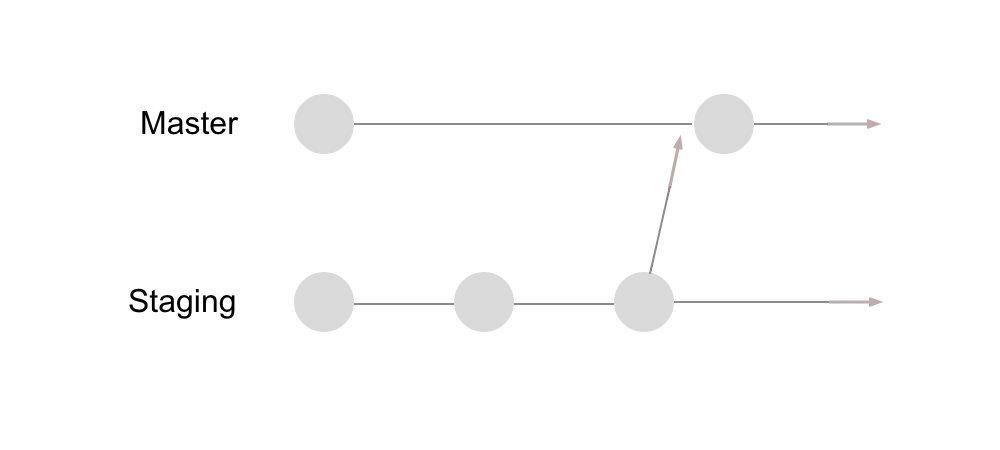
\includegraphics[width=10cm]{master-staging.png}
    \caption{Repozytorium z branchami master oraz staging}
    \label{fig:git}
\end{figure}
Struktura na Gicie dobrze odzwierciedla jakie środowiska mamy. Możemy wykorzystać ten fakt i za pomocą serwera ciągłego dostarczania budować aplikację i automatycznie ją instalować na serwerze stagin'owym za każdym razem, gdy ktoś zrobi commit'a na gałęzi staging. Dzięki takiemu podejściu oszczędzamy czas testerów. Nie muszą oni czekać na techniczną osobę, która zaktualizuje środowisko staging'owe. 
\par
By dalej ułatwić proces wypuszczania oprogramowania możemy zrobić podobne kroki jak przy staging'u dla wersji produkcyjnej. Za każdym razem, gdy ktoś wrzuca nowe zmiany na gałąź master możemy zbudować obraz (więcej o tworzeniu obrazów w rozdziale 2) z serwisem i wysłać go do rejestru obrazów. Tym sposobem kwestia wypuszczenia oprogramowania na serwer produkcyjny zostaje po stronie DevOps'a/administratora, który manualnie może wywołać proces aktualizacji danego serwisu. 
\subsection{Ciągła dystrybucja}
Ciągła dystrybucja jest rozszerzeniem ciągłego dostarczania. Proces ten zakłada, że zmiany, które znajdują się na naszej głównej gałęzi na repozytorium odzwierciedlają stan, który jest na serwerze produkcyjnym. Możemy to osiągnąć poprzez proces budujący aplikacje oraz aktualizujący serwer produkcyjny za każdym razem, gdy ktoś wrzuci nowego commit'a. Podejście to wymaga samodyscypliny i dobrej organizacji w zespole deweloperskim. Zespół musi być świadomy tego, że jeżeli dane zmiany nie są zanadto przetestowane, może to spowodować problemy na środowisku produkcyjnym, które jest kluczowe dla biznesu. W skrajnym przypadku może okazać się, że środowisko produkcyjne będzie działało z problemami przez dłuższy czas i dane, które trzymamy w bazie zostaną "zepsute" przez wadliwy kod.
\par
Problemy te możemy zminimalizować przez stosowanie następujących dobrych praktyk:
\begin{itemize}
    \item Wsteczna kompatybilność - jeżeli dana wersja ma w sobie błąd, administrator serwera w każdej chwili będzie w stanie cofnąć działającą wersję aplikacji do wersji, która nie miała problemów,
    \item Orkiestrator - nowoczesne orkiestratory takie jak np. Kubernetes (o orkiestratorach traktuje rozdział 2) umożliwiają zrobienie tzw. \textit{roll back}(cofnięcia do wcześniejszej wersji) w prosty sposób. Dzięki temu czas, w którym klienci doświadczyli problemów będzie stosunkowo krótki,
    \item Kopia zapasowa bazy danych - dzięki kopii możemy być pewni, że w przypadku "zepsucia" danych lub ich utraty przez błąd w programie będziemy w stanie je odzyskać,
    \item Testy e2e - dodanie testów całościowych systemu jest ważną rzeczą w kontekście ciągłej dystrybucji. Odpalając testy e2e na wersji deweloperskiej aplikacji możemy być bardziej pewni, że zmiany, które zostały dodane, nie psują istniejących funkcjonalności.
\end{itemize}
Dzięki wdrożeniu procesu ciągłej dystrybucji czas między stworzeniem danego kodu i wysłaniem go na repozytorium a uruchomieniem go na środowisku produkcyjnym zmniejsza się. Dodatkowo nie musimy poświęcać czasu administratora by zaktualizować środowisko produkcyjne. Należy pamiętać, że bez odpowiedniej dyscypliny programistów oraz braku stosowania dobrych praktyk proces ciągłej dystrybucji może spowodować więcej problemów niż korzyści. Zazwyczaj proces ten jest stosowany przez doświadczone zespoły deweloperskie.
\subsection{GitOps - czym jest?}
GitOps jest zbiorem dobrych praktyk, opisująca prawidłowy sposób wypuszczania aplikacji na środowisko deweloperskie jak i też produkcyjne. Jest to swoiste rozszerzenie procesu ciągłego dowożenia. Metodologia ta zachęca do trzymania plików konfiguracyjnych danego orkiestratora na repozytorium Git'owym. Dzięki takiej praktyce zyskujemy:
\begin{itemize}
    \item Możliwość weryfikacji jakości zmian, tzw. \textit{Code Review}. Dlatego że konfiguracja jest trzymana na Gicie, inni deweloperzy mogą ocenić, czy nasze zmiany są właściwe. Jest to dość duża zmiana względem tradycyjnego modelu, gdzie administrator sam decydował o zmianach w konfiguracji,
    \item Historię zmian - możemy dzięki temu przejrzeć, jak w przeszłości aplikacja była skonfigurowana,
    \item Przejrzystość systemu - każdy członek techniczny może podejrzeć to, w jaki sposób aplikacja działa na serwerze deweloperskim/produkcyjnym. W modelu tradycyjnym przeciętni członkowie nie wiedzą jak wygląda konfiguracja serwera - dostęp ma tylko administrator,
    \item Automatyzację procesu wypuszczania, czyli ciągłe dowożenie. Jeżeli projekt korzysta z praktyk GitOps, z definicji spełnia proces ciągłego dowożenia. Każda zmiana na gałęzi deweloperskiej/produkcyjnej powoduje to, że wypuszczamy nową wersję oprogramowania na serwerze.
\end{itemize}
\par
Termin GitOps został spopularyzowany przez orkiestrator Kubernetes. Pliki konfiguracyjne Kubernetesa są plikami w formacie YAML. Mocna decentralizacja sposobu, w jakim działa Kubernetes pozwala na trzymanie plików konfiguracyjnych pojedynczych jednostek logicznych w osobnych plikach. Jest to cecha ważna dla projektów opartych o architekturę mikroserwisową. W takich projektach mamy kilkanaście serwisów odpowiedzialnych za różne aspekty biznesowe aplikacji. Każdy taki serwis posiada własne repozytorium kodu w Gicie. Dzięki możliwości decentralizacji plików konfiguracyjnych Kubernetesa możemy dla każdego mikroserwisu trzymać te pliki osobno - każdy mikroserwis ma tylko pliki konfiguracyjne dotyczące samego siebie. Zapewnia to większą separację logiczną. Możność aplikowania na klaster Kubernetesowy pojedynczego pliku YAML, który stanowi tylko częściową konfigurację całego systemu, pozwala na aktualizację tylko pojedynczego serwisu na klastrze. Dzięki temu poszczególne serwisy stają się bardziej niezależne od siebie.
\par
Załóżmy, że tworzymy aplikację opartą na mikroserwisach. Jednym z elementów tej aplikacji jest serwis zarządzający użytkownikami. Serwis ten zajmuje się logiką związaną z zarządzaniem użytkownikami. Jest on stworzony w języku JavaScript i swoją usługę wystawia na porcie 3000. Jego kod wygląda następująco:
\begin{lstlisting}[caption={Serwis zarządzający użytkownikami}]
    const express = require('express')
    const app = express()
    const port = 3000
    const users = [
        {
            name: 'Jan',
            email: 'jan@gmail.com',
        }, 
        {
            name: 'Kasia',
            email: 'kasia@gmail.com',
        }
    ]
    
    app.get('/get-all-users', (req, res) => {
        res.send(users)
    })
    
    app.listen(port, () => {
        console.log(`Users service listening at http://localhost:${port}`)
    })
\end{lstlisting}
Jednym z elementów tego serwisu jest plik konfiguracyjny Kubernetesa, który zajmuje się zdefiniowaniem usługi, jaki nasz serwis ma oferować. Usługa to jeden z obiektów Kubernetesa, który umożliwia przesłanie ruchu sieciowego do instancji z usługą. Plik konfiguracyjny wygląda następująco:
\begin{lstlisting}
kind: Service
apiVersion: v1
metadata:
  name: user-service
  namespace: production
  labels:
    run: user-service
  annotations:
    service.beta.kubernetes.io/aws-load-balancer-internal: 0.0.0.0/0
spec:
  selector:
    app: UserService
  ports:
  - protocol: TCP
    port: 80
    targetPort: 3000
  type: LoadBalancer
\end{lstlisting}
Okazuje się, że z jakiegoś powodu chcielibyśmy zmienić port, na którym nasz serwis z użytkownikami nasłuchuje. W tym celu musimy zmienić plik JavaScript'owy oraz plik YAML z konfiguracją Kubernetesa. Dzięki temu, że obydwa pliki są częścią jednego repozytorium możemy taką zmianę wykonać za pomocą jednego pull request'a. Nie musimy do całej akcji zmiany portu angażować administratora klastra Kubernetesowego - administrator jedyne przegląda, czy nasze zmiany są poprawne. Po zmergowaniu aktualizacja środowiska na klastrze następuje automatycznie. Przebiega to przy użyciu procesu ciągłego dowożenia.
\subsection{Serwery automatyzujące SaaS kontra self-hosted}
We wczesnych latach rozwoju oprogramowania służącego do ciągłej integracji popularność zyskał Jenkins. Jenkins to oprogramowanie, które jest zainstalowane na serwerze i pozwala tworzyć potoki automatyzujące. Może on służyć do stworzenia procesów ciągłej integracji, ciągłego dostarczania oraz ciągłego dowożenia. Jego charakterystyczną cechą jest to, że został on przygotowany do uruchomienia na własnym serwerze - tzw. self-hosted. Instalacja oraz utrzymanie Jenkinsa wymaga czasu specjalisty. Przewaga nad rozwiązaniami typu SaaS (z ang. \textit{oprogramowanie jako usługa}) jest taka, że mamy większą kontrolę nad tym jak Jenkins działa.
Jenkins to nie jedyne rozwiązanie self-hosted do automatyzacji:
\begin{itemize}
    \item CruiseControl - powstał w 2001 roku. Skupiał się na automatyzacji projektów tworzonych w języku Java,
    \item Hudson - prekursor Jenkinsa, który przestał być rozwijany w 2016. Był tworzony jako alternatywa do CruiseControl. W roku 2011 został stworzony fork, którym teraz jest Jenkins,
    \item GitLab CI - jako jeden z nielicznych projektów oferuje możliwość wyboru i używania w formie self-hosted oraz w formie SaaS, dostępnej pod adresem \textit{gitlab.com}. Oprogramowanie to wyróżnia integracja z repozytorium kodu, dzięki której w kilku krokach możemy dodać automatyczne budowanie do naszego projektu. Kod całej platformy GitLab jest dostępny w formie open source.
\end{itemize}
\begin{figure}[htbp]
    \centering
    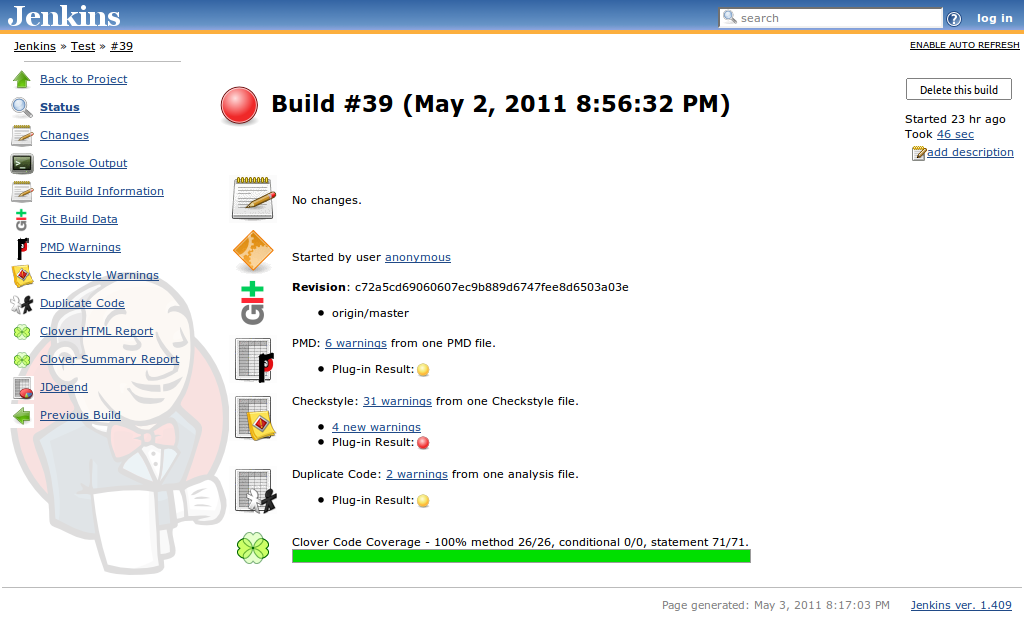
\includegraphics[width=12cm]{jenkins.png}
    \caption{Interfejs webowy Jenkinsa}
    \label{fig:jenkins}
\end{figure}
\par
Lata 10 XXI wieku przyczyniły się do popularyzacji rozwiązań typu SaaS, w których zespół deweloperski nie musi już utrzymywać własnego serwera z zainstalowanym tam oprogramowaniem. Dzięki SaaS utrzymaniem serwera zajmuje się strona trzecia, która za pewną opłatą zapewnia dostęp do aplikacji - zostawiając po swojej stronie sprawy związane z utrzymaniem oraz aktualizacją. Model ten stał się niezwykle popularny dla startup'ów. Firmy takie zazwyczaj posiadają tylko kilkoro ludzi technicznych. Użycie oprogramowania w formie SaaS pozwala takim zespołom skupić się na tworzeniu kodu, który ma dostarczać wartość biznesową. Do najpopularniejszych rozwiązań SaaS do automatyzacji należą:
\begin{itemize}
    \item Travis CI - jest to serwis który zapewnia integrację z repozytorium trzymanym na GitHubie oraz BitBuckecie. Jego kod jest oferowany w formie open source - aczkolwiek jego samodzielna instalacja na własnym serwerze jest dość wymagająca \cite{TravisCI},
    \item GitLab CI - może być używany w postaci SaaS. Oferuje on jedynie integrację z repozytorium hostowanym przez GitLaba,
    \item GitHub Actions - rozwiązanie do automatyzacji zaproponowane przez GitHuba. Zapewnia integrację z repozytorium kodu hostowanym na GitHubie. Jest zamknięto-źródłowym projektem,
    \item CircleCI - rozwiązanie podobne do Travis CI. Różnica polega na tym, że CircleCI zapewnia integrację tylko z repozytorium hostowanym na GitHubie. Dodatkowo jego kod nie jest dystrybuowany w formie open source - jest zamknięty.
\end{itemize}